\chapter[Segmentation and Neural Style Transfer]{Beyond classification and detection: Segmentation, Instance Segmentation,  Neural Style Transfer}

\begin{quotation}
    \noindent
    \textsf{In this chapter we will consider other, even more  complex, computer vision tasks including \textit{semantic segmentation} (the task of classifying each pixel of an image) here encoder-decoder architectures are used, \textit{instance segmentation} (combining object detection and semantic segmentation), \textit{face recognition} using Siamese Network and finally the first step toward the world of generative AI concerning \textit{neural style transfer}.
    }
\end{quotation}

\section{Semantic segmentation}
\textbf{Semantic Segmentation} is the task of labeling each pixel within an image with a \textit{category label} without differentiate instances/object of a certain class. Roughly speaking: I know that a certain pixel of a given image is associated to a cow, but I don't know that there is one or more cow in the image itself. \\
Let us introduce this topic by doing an important observation: since I want to classify each pixel of a given image, the size of the output (width, height) is supposed to be the same as the input. \textbf{What approach can we use?} Let us analyze the problem step by step, following the intuition and then introducing more complex reasonings in order to make the architecture scale up. 

\begin{figure}[h]
    \centering
    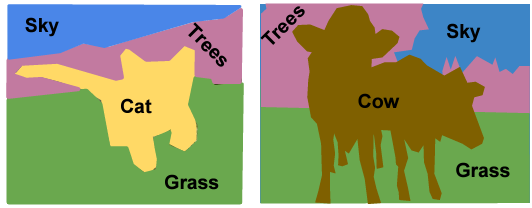
\includegraphics[scale=0.8]{img/Sem_Seg.png}
    \caption{\textbf{Semantic segmentation} Since here I am not able to separate different instances of a given class, I cannot distinguish two cows within the image on the right}
\end{figure}
In the case we want to perform a \textit{semantic segmentation} we can try to use the sliding window approach classifying the center pixel with a ConvNet. How you can image, this approach is extremely inefficient since the image must pass through an entire pipeline until all of its pixels have been classified, without reusing the shared area among the several patches/window. \\
Now, trying to follow the same path as the object detection, we can go toward a \textbf{fully convolutional approach}, since we have to fulfill the requirement on the shape of the output, one could propose to fix 2/3 of the dimension in a way that \emph{height and width} can have the same shape across the convolutional layers. This solution does not scale on the input size, for this reason new models are used called \textbf{encoder-decoder} that downsample and then \textbf{upsample} in the second part of the network in order to match the input size by using: (i) \textit{in-network upsampling} (\textbf{unpooling}), (ii) \textit{learnable upsampling} (\textbf{deconvolution or transpose convolutions}) (both these aspects are explained in \cite{noh2015learning}).

\subsection{In-Network upsampling: Unpooling}
The \textit{pooling} operation in convolutional networks helps us to filter \textbf{non-robust activation} by keeping a single (max/average...) representative value. However all the spatial information about such a value is lost. In order to solve such an issue the unpooling layer is employed into the deconvolutional part of the network (decoder) is used. The unpooling perform the \textbf{reverse operation of pooling} and reconstruct the original size of activations. Some \textbf{switch variables} are used in order to store the location of the maximum activation as showed in the following: 

\begin{figure}[h]
    \centering
    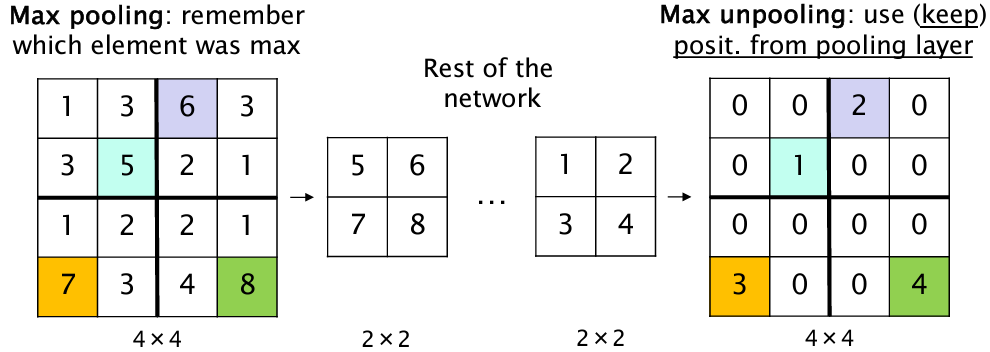
\includegraphics[scale=0.5]{img/Unpooling.png}
\end{figure}
The first part and second part of such an architecture are simmetric, so that the pooled and unpooled layers are specular. 

\begin{multicols}{2}
    \begin{center}
        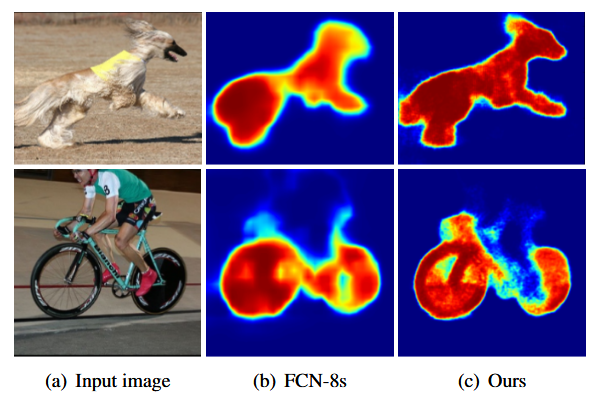
\includegraphics[scale=0.5]{img/FCNvsED.png}
        Activation maps from FCN and Encoder-Decoder architecture
    \end{center}
    \begin{center}
        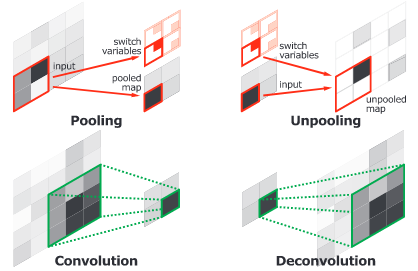
\includegraphics[scale=0.8]{img/Unpool_Deconv.png}
        Pooling/Unpooling and Convolution/Deconvolution
    \end{center}
\end{multicols}

\subsection{Learnable upsampling: Deconvolution}
When the unpooling operation is applied we retrieve an \textbf{enlarged} but \textbf{sparse} map. The main role of the \textit{deconvolutional part} of an encoder is to \textbf{densify the sparse activations} obtained by unpooling. How the \Cref{fig: deconv_unpool} shows, the deconvolution operation maps a single input into multiple outputs. Several \textit{learnable deconvolutional filters} are used which have a similar function with respect to the convolutional one. Lower layers are likely to capture the shape of the overall object while the deeper one will the capture other \textit{fine details}. In this way the decoder \textbf{directly takes class-specific shape information into account}.\\
The \textbf{transpose convolution} operation takes the input feature map and multiply a certain value for all the value contained in the filter so that the important information from the encoder are spread back; in the overlapped region takes as activation the sum of the numbers. In conclusion as in the case of "normal" convolution there are some hyperparameters (filter dimensions and stride).\footnote{Going more deeply, we can say that \emph{"...unpooling and deconvolution play different roles for the construction ot segmentation masks. Unpooling captures \underline{example-specific} by tracing the original locations (with strong activations) back to the image space. As a result, it effectively reconstructs the detailed structure of an object in finer resolutions. On the other hand, learned filters in deconvolutional layers tend to capture \underline{class-specific} shapes. Through deconvolutions, the activations closely related to the target classes are amplified while noisy activations from other regions are suppressed effectively. By the combination of unpooling and deconvolution, our network generates accurate segmentation maps."}(from \citeauthor{noh2015learning} \cite{noh2015learning}).}

\subsection{SegNet: Encoder-Decoder for Image Segmentation}
SegNet (\citeauthor{badrinarayanan2017segnet} \cite{badrinarayanan2017segnet}) introduces a more robust way to segment a given image without the necessity to deconvolve it, on the contrary it uses 'normal' convolutional filters. Those that in \citeauthor{noh2015learning} (\cite{noh2015learning}) are called \textit{switch variables}, here are called \textit{max-pooling indexes}. The underlying concept is the same: keep unchanged the position of the most important information.

\begin{figure}[h]
    \centering
    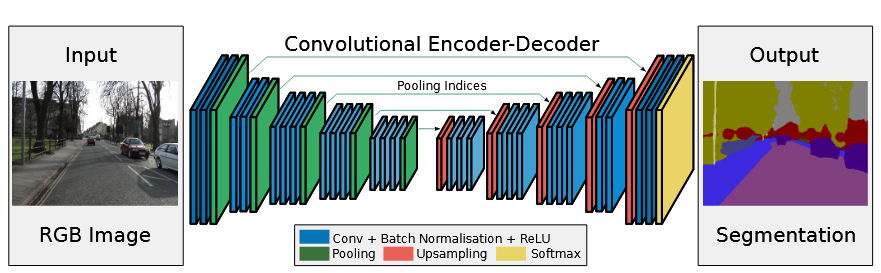
\includegraphics[scale=0.7]{img/SegNet.png}
    \caption{SegNet architecture}
\end{figure}

The performance of such a network is even better with the respect to the one presented before, due to the simpler method employed for upsampling. At the end of the decoder convolutional layer, logits are passed through a softmax layer in order to obtain \textbf{probabilities}. After that we compute the class by doing the max. \textbf{Each class is associated with a specific color}, this by doing post-processing is transformed into a \textbf{color-coded segmentation map}. \Cref{tab:segVSnoh} shows a comparison between the Deconvolution Network and Seg-Net.

\begin{table}
\centering
\begin{tabular}{|>{\raggedright\arraybackslash}p{4cm}|>{\raggedright\arraybackslash}p{5cm}|>{\raggedright\arraybackslash}p{5cm}|}
\hline
\textbf{Feature}                  & \textsc{Deconvolution Network}     & \textsc{SegNet}                           \\ \hline
\textbf{Guiding Spatial Information} & Switch variables (max-pooling indices)         & Max-pooling indices                        \\ \hline
\textbf{Upsampling Method}         & Unpooling + Deconvolution (transpose convolutions) & Unpooling                                  \\ \hline
\textbf{Convolution Type in Decoder} & Transpose convolutions (learnable filters)     & Normal convolutions (learnable filters)    \\ \hline
\textbf{Output of Unpooling}       & Sparse feature map                              & Sparse feature map                         \\ \hline
\textbf{Densification Process}     & Deconvolution spreads activations and learns filters & Normal convolutions refine feature maps    \\ \hline
\textbf{Complexity}                & Higher (learnable upsampling)                   & Lower (fixed unpooling, separate convolutions) \\ \hline
\end{tabular}
\caption{Comparison between Noh et al. (Deconvolution Network) and SegNet.}
\label{tab:segVSnoh}
\end{table}

\subsection{Other Architectures for segmentation}

\subsubsection{\textsf{U-Net: a framework for semantic segmentation in fine-grained domains}}
\textbf{U-Net} (\citeauthor{ronneberger2015u} \citeauthor{ronneberger2015u}) is a ConvNEt designed for \textit{biomedical image segmentation}, but this is not a restriction since can be used also in other fields. Its name is due the \textbf{U-shaped structure} with two parts: encoder (pooling and convolution) and decoder (unpooling and transposed convolutions). Also here \textbf{skip connections} are used in order to preserve spatial information with the guide the upsampling process. Such a network works well also with \textit{small datasets} and is effective for segmentation tasks with \textit{fine structures and boundaries}.

\subsubsection{\textsf{E-Net: real-time semantic segmentation}}
\textbf{E-Net} (\citeauthor{paszke2016enet} \cite{paszke2016enet}) is a neural network taylored for \textbf{real-time semantic segmentation} especially on \textbf{mobile} and \textbf{embedded devices}. Due to the context in which is used and the devices on which it has to run, the architecture is \textit{highly optimized} introducing novelties (asymmetric encoder-decoder, dilated convolutions, pyramid pooling).
    
\section{Instance segmentation}
\begin{figure}[h]
    \centering
    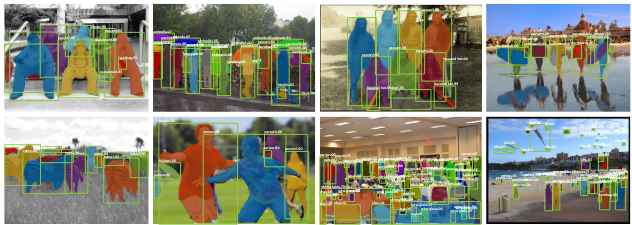
\includegraphics[scale=0.8]{img/InstanceSeg.png}
\end{figure}

\textbf{Instance Segmentation} is an advanced deep learning task which combines \textit{object detection} and \textit{semantic segmentation}: here we want to label in the image with a category label, moreover we want differentiate instances of a given class. \\
The work in which such a technique was presented is called \textsc{Mask R-CNN} (\citeauthor{he2017mask}, \citedate{he2017mask}, \cite{he2017mask}). This extends the \textsc{Faster R-CNN} architecture by adding a branch for \textit{predicting sementation masks for each RoI}. The main stages are kept, in particular the same Region Proposal Network is used and Fast R-CNN in order to classify each RoI. 

\subsection{Segmentation mask}
The difference here is that \underline{in the second stage}, in parallel, to bounding boxes and class prediction there is also a \textbf{binary segmentation map} for each proposal extracted by RPN. \\
A mask contains information about the spatial layout of an object, for this the mask prediction is done by using a fully convolutional network that preserve pixel-per-pixel features.\\
Keep in mind that the output mask is not a direct representation of pixels, it is a low-resolution mask of the object for the given RoI, then it is upsampled in order to meet the original dimensions (for example if the RoI spans an area of $56\times56$ and the extracted mask is $14\times14$, then it will be upsampled to $56\times56$). The upsampled mask contains continuous values ranging from 0 to 1, a certain threshold is used in order to keep/discard the values.

\begin{multicols}{2}
    \begin{center}
        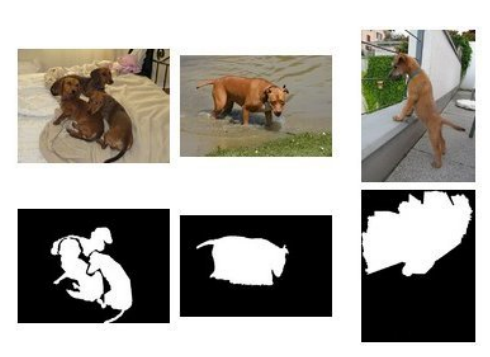
\includegraphics[scale=0.7]{img/seg.png}
        Segmentation mask examples
    \end{center}
    \newcolumn
    \begin{center}
        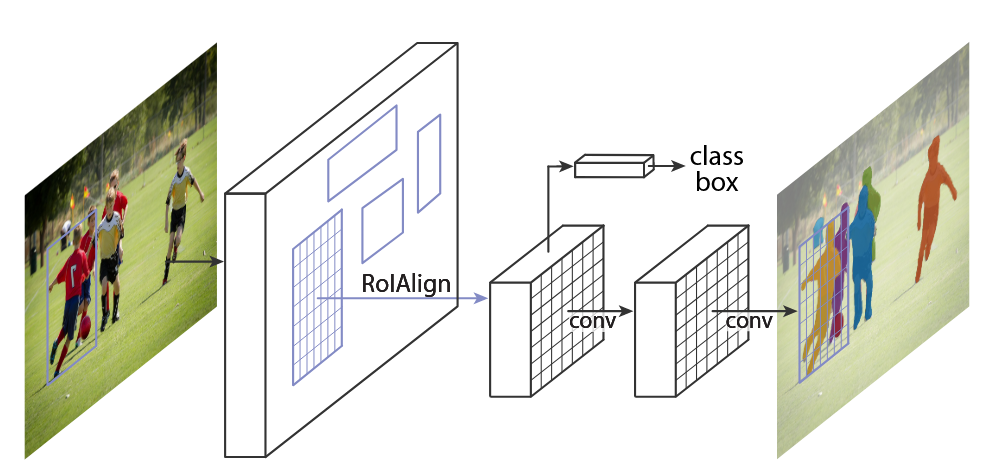
\includegraphics[scale=0.4]{img/maskRCNN.png}\\
        \textbf{Mask R-CNN architecture}
    \end{center}
\end{multicols}

\subsection{RoI-Align}
Since a segmentation mask need to preserve spatial information, it is needed that the RoI features are faithfully coherent with the layout of a certain image. \\
In \textsc{Fast R-CNN} and \textsc{Faster R-CNN}, RoI pooling is used in order to extract the main features from the region proposals. An harsh quantization effect is introduced by RoI pooling which surely results in lack of important information that here are crucial! \textit{RoI Align} method introduced in \cite{he2017mask} avoid such effects by aligning the RoI feature maps.\footnote{
    By using \textit{bilinear interpolation methods}. See the article for more detailed information
}


\subsection{Traing Mask R-CNN}
Similarly than the Faster R-CNN, here a \textit{multi-task loss} is employed on each sampled RoI which has the following structure:

\begin{equation}
    L = L_{cls}+L_{box}+L_{mask}
\end{equation}
\noindent
where $L_{mask}$ is the cost function part devoted to the mask prediction, in particular a binary cross entropy loss is used and clearly a per-pixel prediction is done.\\

\noindent
In conclusion, we can add a further detail. Following the same road we have done till now, we could ask to the network to learn other information like \textbf{joint positions}, clearly complexity is added to the network structure. More complex and complete labeled datasets are used in order to train such even more complex architectures.

\section{Face verification/recognition}
\begin{figure}[h]
    \centering
    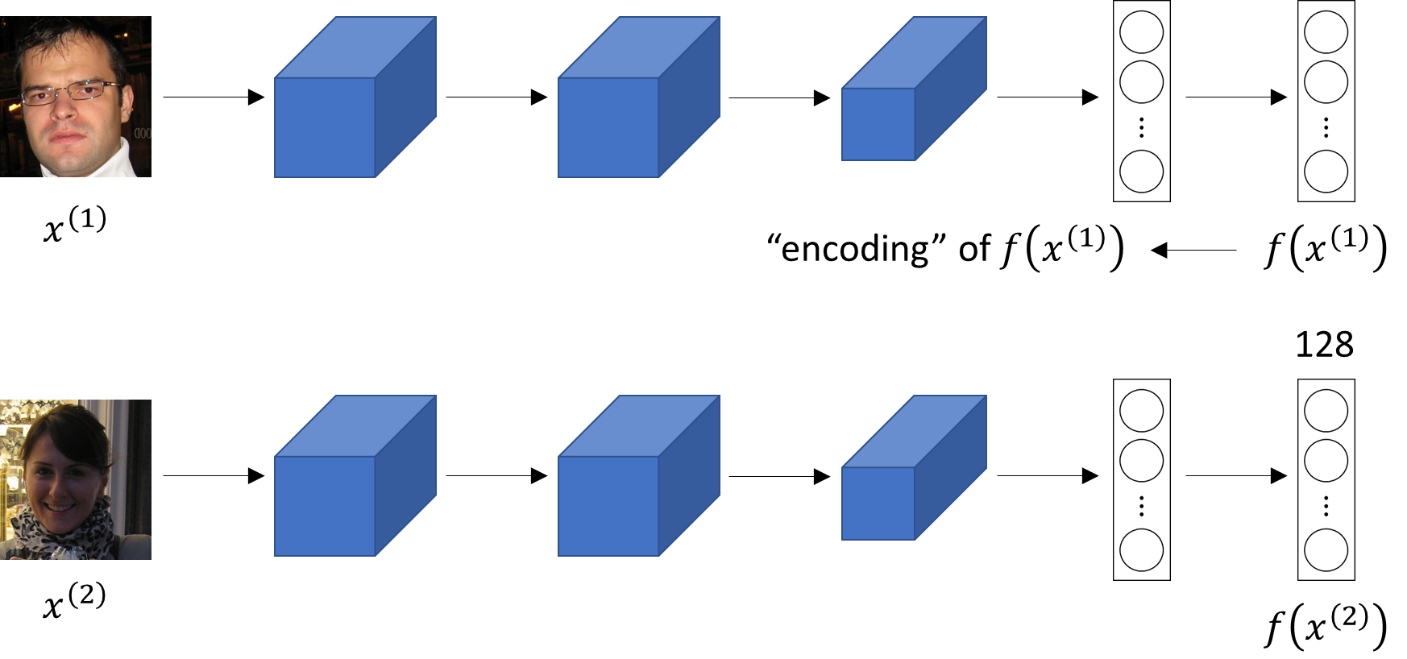
\includegraphics[scale=0.6]{img/face_recognition.png}
    \caption{Face recognition}
\end{figure}

\noindent
Here we introduce two similar computer vision task: (i) \textit{face verification}, that deals with saying wheter a given image owns to a given person; (ii) \textit{face recognition} where given a database of $K$ people and given an input image, the task is saying given a new sample if that image is any of the $K$ people in the database. The related work is \textit{\citetitle{schroff2015facenet}} (\cite{schroff2015facenet}). 
In this field is common to introduce the concept of \textbf{single shot learning} which is the task of learning from one example to recognize a given person again.

\subsection{The need of a similarity function}
Here we need a \textbf{similarity function} between two images, a sort of distance $d$(img1, img2) so that we can use it for both verification and recognition. In the first case we can use a threshold $\tau$ since the output is YES/NO, in the second part we can output the person identity whose image distance with the input is minimized.\\
In the context of ConvNets we know that passing through a generic image sample $x^{(1)}$ in the last layer before softmax is a vector of features (\textbf{embedding vector}), that we can call $f(x^{(1)})$. Now, given two images $x^{(1)}$ and $x^{(2)}$, we can compute a distance as:
\begin{equation}
    d(x^{(1)}, x^{(2)})=\Vert f(x^{(1)}) - f(x^{(2)}) \Vert_2^2 
\end{equation}
The network is supposed to learn parameters so that such a distance is small if the two images are related to the same people, otherwise it is larger.

\subsection{Triplet loss}
The so-called \textbf{triplet loss function} is more suitable for face recognition, the main motivation is that other loss functions try to project a given sample on a single point, the triplet loss -- instead -- tries to enforce a margin of difference.\\
In this context we want to ensure that an image $x_i^{a}$ anchor of a specific person is closer to all other images $x_i^{p}$ of the same people than it is is with respect to the other images $x_i^{n}$ of other people. More specifically we want that:
\begin{equation}
    \Vert f(x_i^{p})-f(x_i^{a}) \Vert_2^2 + \alpha <
    \Vert f(x_i^{a})-f(x_i^{n}) \Vert_2^2 \quad 
    \forall \big(
        x_i^{p}, x_i^{a}, x_i^{n}
    \big) \in \mathcal{T}
\end{equation}
where $\mathcal{T}$ is the set of all the triplets in the training set and has cardinality $N$. The loss function to be minimized in this context is:
\begin{equation}
    \mathcal{L}=\sum_i^{N} {
        \big[
            \Vert f(x_i^{p})-f(x_i^{a}) \Vert_2^2 - \Vert f(x_i^{a})-f(x_i^{n}) \Vert_2^2 + \alpha
        \big]
    }
\end{equation}
The triplets must be chosen in a way that the inequality is not satisfied in the great majority of the cases. In the cited paper \cite{schroff2015facenet} there is an entire section devoted to how properly select the triplets of the set $\mathcal{T}$.


\begin{figure}
    \centering
    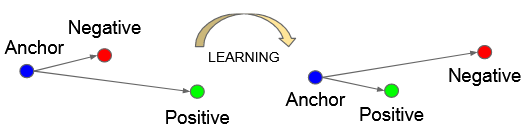
\includegraphics[scale=0.8]{img/triplet.png}
    \caption{Triplet loss objective}
\end{figure}

\subsection{Siamese Network}
A \textbf{Siamese Network} is a class of neural network architectures that \textbf{contain two or more \textit{identical} subnetworks}, in the sense they share the same configuration, but also the same set of parameters. Siamese networks learn a similarity function, and they can be used together with binary classification to learn similarities. Here we have an example: 

\begin{figure}[h]
    \centering
    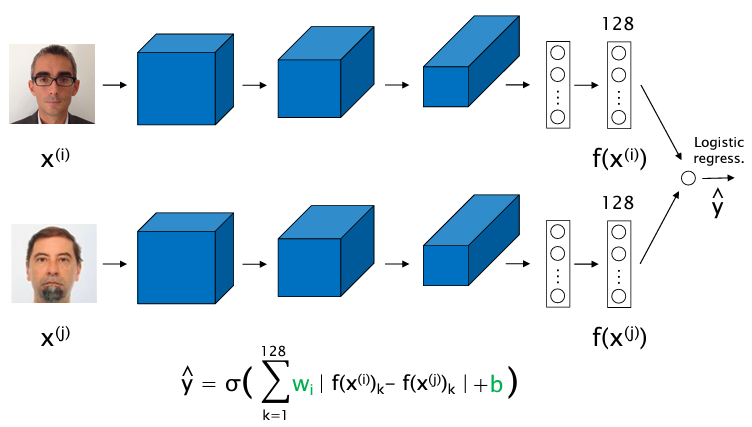
\includegraphics[scale=0.7]{img/siamese_2.png}
    \caption{Siamese network}
\end{figure}
The parameters $w_i$ and $b$ are learnt for the pair of networks. The single network is trained using the triplet loss that -- summarizing -- maps each image of the input in a space of embeddings where similar faces are closer than different faces.

\section{Neural style transfer}
Now we present a technique which is the first step toward the generative AI techniques. The main reference for this part is \textit{\citetitle{gatys2015neural} \cite{gatys2015neural}}. Essentially the objective here is to generate a new image that could have:
\begin{itemize}
    \itemsep-0.2em
    \item The \textbf{content (C)}, that is the structure, of a certain image;
    \item The \textbf{style (S)}, from another image.
\end{itemize}

\begin{figure}[h]
    \centering
    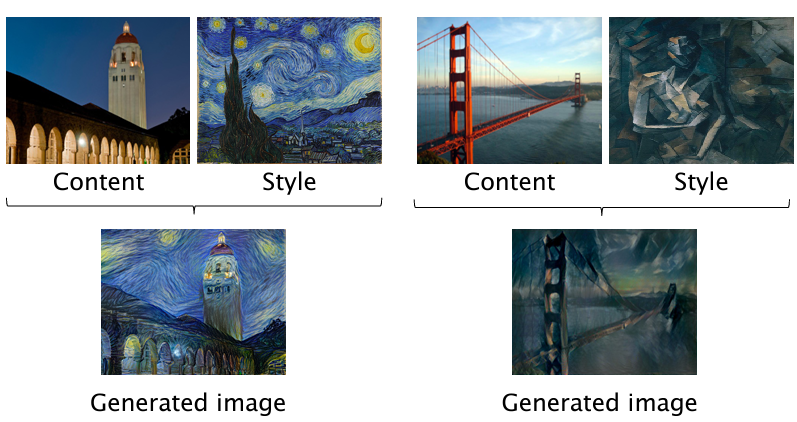
\includegraphics[scale=0.7]{img/NeuralStyle.png}
    \caption{Neural Transfer Style}
\end{figure}

Before entering into more details, it is crucial dedicate few words on the type of information a convolutional network is able to learn at different layers. We can say that high level details about the structure (\textbf{content}) is learnt at deeper layers while \textit{low level details} like textures and patterns related to the \textbf{style}, are mapped into the initial layers. \\

\noindent
The cost function to be used in such a context is a \textit{multi-task} one like: 
\begin{equation}
    J(G)=\alpha{J_{\text{Content}}(C,G)+\beta{J_{\text{Style}}(S,G)}}
\end{equation}
where $G$ is referred to the \textbf{generated image}. Let us see more deeper what is the structure of the functional part related to the content and to the style.

\subsection{$J_{\text{Content}}(C,G)$: content cost function}
In order to compute the cost function we sample the activations of the network at a certain layer $l$, let $a^{[l](C)}$ and $a^{[l](G)}$ be the activation of a certain network structure computed on the content image and on the generated image. Such activations are similar if both images have similar content. Then, the functional related to the content is:

\begin{equation}
    J_{\text{Content}}(C,G)=\frac{1}{2} \Vert a^{[l](C)}-a^{[l](G)} \Vert_2^2
\end{equation}

\subsection{$J_{\text{Style}}(S,G)$: style cost function}
As it us stated in \cite{gatys2015neural} the style of an image can be computed as the existing correlation among different channels of a certain layer $l$. These can be expressed in term of the \textit{Gramian matrix} of the layer $l$ itself. For the style image, I take the activations of the layer $l$ and I compute the matrix $G^{[l](S)}$ where the entry $G_{ij}$ is:
\begin{equation}
    G_{ij}=\sum_{k} {F_{i,k}\cdot F_{j,k}}
\end{equation}

Practically speaking given the activation tensor of a certain layer $G^{[l](S)}$ can be computed in the following way: 
\begin{itemize}
    \itemsep-0.2em
    \item Given the tensor $n_H\times{n_{W}}\times{n_{C}}$, we have to perform the reshape $n_{C}\times({n_{H}\times{n_{W}}})$ by unrolling in a row vector the matrix associated in a channel and then composing them by row.
    \item The matrix $G^{[l](S)}$ can be computed by multiplying this intermediate matrix by its transpose.
\end{itemize}
At this point, we are to give (approximately) the structure for the style cost function:
\begin{equation}
    J^{[l]}_{\text{Style}}(S,G)=\Vert G^{[l](S)}-G^{[l](G)} \Vert_F^2
\end{equation}
Since for the style several layers are considered the final shape is:
\begin{equation}
    J_{\text{Style}}(S,G)=\sum_{l}{ \lambda^{[l]} J^{[l]}_{\text{Style}}(S,G)}
\end{equation}
where $\lambda^{[l]}$ are the weights for the different layers.

\subsection{Generating the output image}
The output image is generated in the following way:
\begin{enumerate}
    \itemsep-0.2em
    \item Given $C$ and $S$, initialize $G$ randomly or starting by the content image; 
    \item Gradient Descent is used in order to minimize the cost function $J(G)$ 
\end{enumerate}
An example is shown in the following figure:
\begin{figure}[h]
    \centering
    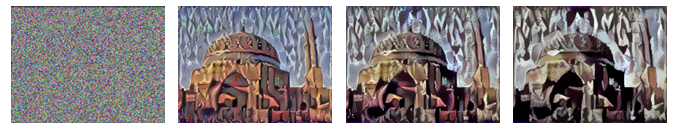
\includegraphics[scale=1]{img/NeuralStyle_G.png}
    \caption{Generating the output image}
\end{figure}

\subsection{Final comments}
Note that an architecture like VGG-16 can be used in order to perform the task, we do not absolutely care about the classification that such a network provides us, since we use it only as a \textbf{feature extractor}. In the practice, given the content and style images, we pass them through the network in order to sample the activations we need in order to compute the loss. After having suitably initialized the generated output, we pass it many times through the network updating it according to the partial derivatives of $J(G)$. 


 






%\section{Dataset for Computer Vision tasks (CV tasks)}